%% Based on a TeXnicCenter-Template by Gyorgy SZEIDL.
%%%%%%%%%%%%%%%%%%%%%%%%%%%%%%%%%%%%%%%%%%%%%%%%%%%%%%%%%%%%%

%------------------------------------------------------------
%
\documentclass{article}%
%Options -- Point size:  10pt (default), 11pt, 12pt
%        -- Paper size:  letterpaper (default), a4paper, a5paper, b5paper
%                        legalpaper, executivepaper
%        -- Orientation  (portrait is the default)
%                        landscape
%        -- Print size:  oneside (default), twoside
%        -- Quality      final(default), draft
%        -- Title page   notitlepage, titlepage(default)
%        -- Columns      onecolumn(default), twocolumn
%        -- Equation numbering (equation numbers on the right is the default)
%                        leqno
%        -- Displayed equations (centered is the default)
%                        fleqn (equations start at the same distance from the right side)
%        -- Open bibliography style (closed is the default)
%                        openbib
% For instance the command
%           \documentclass[a4paper,12pt,leqno]{article}
% ensures that the paper size is a4, the fonts are typeset at the size 12p
% and the equation numbers are on the left side
%
\usepackage{amsmath}%
\usepackage{amsfonts}%
\usepackage{amssymb}%
\usepackage{graphicx}%
\usepackage{tabularx}%
\usepackage{epstopdf}

\addtolength{\textheight}{3.2cm}
\addtolength{\textwidth}{2.6cm}
\addtolength{\marginparwidth}{-2.2cm}
\addtolength{\oddsidemargin}{-1.2cm}
\addtolength{\headheight}{-2.4cm}

%-------------------------------------------
\newtheorem{theorem}{Theorem}
\newtheorem{acknowledgement}[theorem]{Acknowledgement}
\newtheorem{algorithm}[theorem]{Algorithm}
\newtheorem{axiom}[theorem]{Axiom}
\newtheorem{case}[theorem]{Case}
\newtheorem{claim}[theorem]{Claim}
\newtheorem{conclusion}[theorem]{Conclusion}
\newtheorem{condition}[theorem]{Condition}
\newtheorem{conjecture}[theorem]{Conjecture}
\newtheorem{corollary}[theorem]{Corollary}
\newtheorem{criterion}[theorem]{Criterion}
\newtheorem{definition}[theorem]{Definition}
\newtheorem{example}[theorem]{Example}
\newtheorem{exercise}[theorem]{Exercise}
\newtheorem{lemma}[theorem]{Lemma}
\newtheorem{notation}[theorem]{Notation}
\newtheorem{problem}[theorem]{Problem}
\newtheorem{proposition}[theorem]{Proposition}
\newtheorem{remark}[theorem]{Remark}
\newtheorem{solution}[theorem]{Solution}
\newtheorem{summary}[theorem]{Summary}
\newenvironment{proof}[1][Proof]{\textbf{#1.} }{\ \rule{0.5em}{0.5em}}

\begin{document}

\title{Department of  Statistics \\ STATS 784: Data Mining}
\author{Zhi Zhang, $\ $708439475, $\ $zzha822
\\The University of Auckland}
\date{Sep 16th, 2017}
\maketitle

%\begin{abstract}
%This is a sample document which shows the most important features of the Standard
%\LaTeX\ Journal Article class.
%\end{abstract}

\section{Question 1}
\subsection{ROC curve definition and interpretation}
\textbf{Receiver Operating Characteristic} (\textbf{ROC}) curves were designed as a general method that, given a collection of continuous data points, determine an effective threshold such that values above the threshold are indicative of a specific event. \\
\indent Generally the ROC curve is one technique for evaluating the trade-off between \emph{Sensitivity} and \emph{Specificity}, which are used to evaluate the two-class problem in classification model, such as logistic regression. The sensitivity of the model is the rate that the event
of interest is predicted correctly for all samples having the event, which is sometimes considered as the \emph{true positive} rate since it measures the accuracy in the event population. Conversely, the specificity is defined as the rate that nonevent samples are predicted as nonevents, and the \emph{false-positive} rate is defined as one minus the specificity. The sensitivity and specificity can be combined into a single value by using the ROC curve.\\
\indent The ROC curve is created by evaluating the class probabilities for the model across a continuum of thresholds. For each candidate threshold, the resulting true-positive rate (i.e., the sensitivity) and the false-positive rate (one minus the specificity) are plotted against each other. This plot is a helpful tool for choosing a threshold that appropriately maximizes the trade-off between sensitivity and specificity.\\
\indent The ROC curve can also be used for a quantitative assessment of the model. A perfect model that completely separates the two classes would have 100\% sensitivity and specificity. Graphically, the ROC curve would be a single step between (0, 0) and (0, 1) and remain constant from (0, 1) to (1, 1). The area under the ROC curve for such a model would be one. A completely ineffective model would result in an ROC curve that closely follows the $45^{\circ}$ diagonal line and would have an area under the ROC curve of approximately 0.50. To visually compare different models, their ROC curves can be superimposed on the same graph. Comparing ROC curves can be useful in contrasting two or more models with different predictor sets (for the same model), different tuning parameters (i.e., within model comparisons), or complete different classifiers (i.e., between models). The optimal model should be shifted towards the upper left corner of the plot. Alternatively, the model with the largest area under the ROC curve would be the most effective.\\
\indent One advantage of using ROC curves to characterize models is that, since it is a function of sensitivity and specificity, the curve is insensitive to disparities in the class proportions. A disadvantage of using the area under the curve to evaluate models is that it obscures
information. For example, when comparing models, it is common that no individual ROC curve is uniformly better than another (i.e., the curves cross). By summarizing these curves, there is a loss of information, especially if one particular area of the curve is of interest. For example, one model may produce a steep ROC curve slope on the left but have a lower AUC (Area Under Curve) than another model. If the lower end of the ROC curve was of primary interest, then AUC would not identify the best model. The partial area under the ROC curve is an alternative that focuses on specific parts of the curve.\\
\indent The ROC curve is only defined for two-class problems but has been extended to handle three or more classes. Hand and Till (2001), Lachiche and Flach (2003), and Li and Fine (2008) use different approaches extending the definition of the ROC curve with more than two classes.

\subsection{ROC curve example}
There are several packages in R can draw ROC curve, such as ROCR, caTools, pROC, etc. Here we will use the roc function in pROC package to draw the ROC curve for logistic regression model of the credit card default in ISLR.
\begin{verbatim}> library(ISLR)
> data(Default)
> default.logistic = glm(default ~ student + balance + income,
+                        data = Default,
+                        family = binomial)
> coef(default.logistic)
  (Intercept)    studentYes       balance        income
-1.086905e+01 -6.467758e-01  5.736505e-03  3.033450e-06
>
> probs = predict(default.logistic, type = "response")
> my.table = table(Default$default, probs > 0.5)
>
> class.sensi = function(table) {
+   table[2,2] / sum(table[2,])
+ }
>
> class.speci = function(table) {
+   table[1,1] / sum(table[1,])
+ }
>
> total.error = function(table) {
+   1 - sum(diag(table)) / sum(table)
+ }
>
> total.error(my.table)
[1] 0.0268
> class.sensi(my.table)
[1] 0.3153153
> class.speci(my.table)
[1] 0.9958622
>
> my.table = table(Default$default, probs > 0.1)
> total.error(my.table)
[1] 0.0645
> class.sensi(my.table)
[1] 0.7447447
> class.speci(my.table)
[1] 0.942071
>
> library(pROC)
> rocCurve = roc(response = Default$default,
+                predictor = probs,
+                levels = rev(levels(Default$default)))
>
> auc(rocCurve)
Area under the curve: 0.9496
> ci.auc(rocCurve)
95% CI: 0.9402-0.959 (DeLong)
>
> par(mfrow = c(1,2))
> plot.roc(rocCurve)
> plot(rocCurve, legacy.axes = TRUE)
> \end{verbatim}
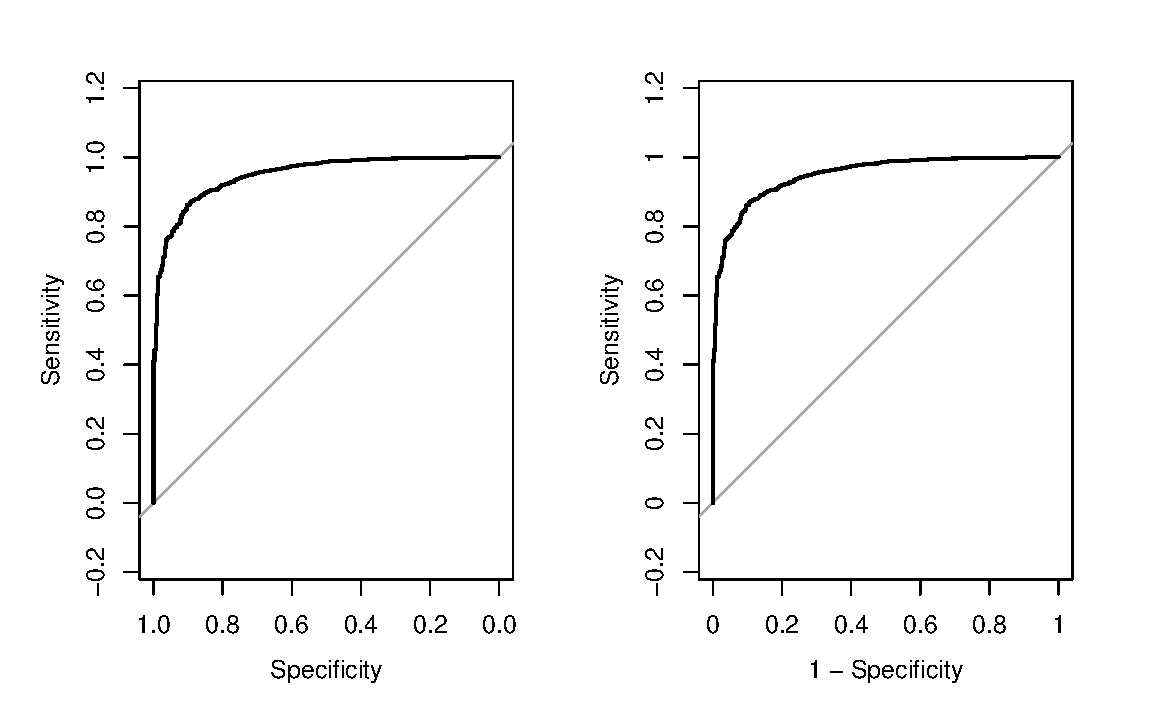
\includegraphics[width=\textwidth]{Rplot_roc_curve.eps}

%\noindent The front matter has various entries such as\\
%\hspace*{\fill}\verb" \title", \verb"\author", \verb"\date", and
%\verb"\thanks"\hspace*{\fill}\\
%You should replace their arguments with your own.
%
%This text is the body of your article. You may delete everything between the commands\\
%\hspace*{\fill} \verb"\begin{document}" \ldots \verb"\end{document}"
%\hspace*{\fill}\\in this file to start with a blank document.


\section{Question 2}
\subsection{Pre-process data}
First we load the voice data from the URL and check if any feature has missing data.
\begin{verbatim}
> voiceURL = "https://www.stat.auckland.ac.nz/~lee/784/Assignments/voice.csv"
> input.df = read.csv(voiceURL, header = TRUE)
> head(input.df)
    meanfreq         sd     median         Q25        Q75        IQR      skew
1 0.05978098 0.06424127 0.03202691 0.015071489 0.09019344 0.07512195 12.863462
2 0.06600874 0.06731003 0.04022873 0.019413867 0.09266619 0.07325232 22.423285
3 0.07731550 0.08382942 0.03671846 0.008701057 0.13190802 0.12320696 30.757155
4 0.15122809 0.07211059 0.15801119 0.096581728 0.20795525 0.11137352  1.232831
5 0.13512039 0.07914610 0.12465623 0.078720218 0.20604493 0.12732471  1.101174
6 0.13278641 0.07955687 0.11908985 0.067957993 0.20959160 0.14163361  1.932562
         kurt    sp.ent       sfm       mode   centroid    meanfun     minfun    maxfun
1  274.402906 0.8933694 0.4919178 0.00000000 0.05978098 0.08427911 0.01570167 0.2758621
2  634.613855 0.8921932 0.5137238 0.00000000 0.06600874 0.10793655 0.01582591 0.2500000
3 1024.927705 0.8463891 0.4789050 0.00000000 0.07731550 0.09870626 0.01565558 0.2711864
4    4.177296 0.9633225 0.7272318 0.08387819 0.15122809 0.08896485 0.01779755 0.2500000
5    4.333713 0.9719551 0.7835681 0.10426140 0.13512039 0.10639784 0.01693122 0.2666667
6    8.308895 0.9631813 0.7383070 0.11255543 0.13278641 0.11013192 0.01711230 0.2539683
      meandom    mindom    maxdom   dfrange    modindx label
1 0.007812500 0.0078125 0.0078125 0.0000000 0.00000000  male
2 0.009014423 0.0078125 0.0546875 0.0468750 0.05263158  male
3 0.007990057 0.0078125 0.0156250 0.0078125 0.04651163  male
4 0.201497396 0.0078125 0.5625000 0.5546875 0.24711908  male
5 0.712812500 0.0078125 5.4843750 5.4765625 0.20827389  male
6 0.298221983 0.0078125 2.7265625 2.7187500 0.12515964  male
>
> apply(input.df, 2, function(x) sum(is.na(x)))
meanfreq       sd   median      Q25      Q75      IQR     skew     kurt   sp.ent      sfm
       0        0        0        0        0        0        0        0        0        0
    mode centroid  meanfun   minfun   maxfun  meandom   mindom   maxdom  dfrange  modindx
       0        0        0        0        0        0        0        0        0        0
   label
       0
> \end{verbatim}
So, no feature has missing data, the we don't need to do imputation for the data. Next, we will scale and symmetrize the data for each appropriate feature.
\begin{verbatim}
> library(caret)
> input.df$label = factor(input.df$label)
> numericCols = unlist(lapply(input.df, is.numeric))
> dataCont = input.df[, numericCols]
> dataFactor = as.data.frame(input.df[, !numericCols])
> names(dataFactor) = names(input.df)[!numericCols]
> trans = preProcess(dataCont,
+                    method = c("BoxCox", "center", "scale"))
> dataTransScaleCont = predict(trans, dataCont)
> dataTransScaled = data.frame(
+   as.data.frame(scale(dataTransScaleCont)),
+   dataFactor)
> str(dataTransScaled)
'data.frame':	3168 obs. of  21 variables:
 $ meanfreq: num  -4.049 -3.84 -3.463 -0.992 -1.53 ...
 $ sd      : num  0.427 0.612 1.604 0.9 1.322 ...
 $ median  : num  -4.224 -3.999 -4.095 -0.759 -1.677 ...
 $ Q25     : num  -2.576 -2.486 -2.707 -0.901 -1.268 ...
 $ Q75     : num  -5.693 -5.588 -3.928 -0.711 -0.792 ...
 $ IQR     : num  -0.215 -0.258 0.909 0.633 1.005 ...
 $ skew    : num  2.293 4.547 6.513 -0.45 -0.481 ...
 $ kurt    : num  1.763 4.432 7.325 -0.24 -0.239 ...
 $ sp.ent  : num  -0.0391 -0.0652 -1.0836 1.5161 1.7081 ...
 $ sfm     : num  0.472 0.594 0.398 1.797 2.114 ...
 $ mode    : num  -2.14 -2.14 -2.14 -1.05 -0.79 ...
 $ centroid: num  -4.049 -3.84 -3.463 -0.992 -1.53 ...
 $ meanfun : num  -1.81 -1.08 -1.37 -1.67 -1.13 ...
 $ minfun  : num  -1.098 -1.091 -1.1 -0.989 -1.034 ...
 $ maxfun  : num  0.566 -0.294 0.41 -0.294 0.26 ...
 $ meandom : num  -1.564 -1.562 -1.564 -1.195 -0.222 ...
 $ mindom  : num  -0.708 -0.708 -0.708 -0.708 -0.708 ...
 $ maxdom  : num  -1.431 -1.418 -1.429 -1.274 0.124 ...
 $ dfrange : num  -1.419 -1.406 -1.417 -1.261 0.137 ...
 $ modindx : num  -1.455 -1.014 -1.065 0.614 0.289 ...
 $ label   : Factor w/ 2 levels "female","male": 2 2 2 2 2 2 2 2 2 2 ...
> \end{verbatim}
It seemed all the voice data have already been symmetrized. Then we will check if any features are correlated or unrelated to the target.
\begin{verbatim}
> colnum = ncol(dataTransScaled)
> cors = cor(dataTransScaled[, 1:(colnum - 1)])[1:(colnum - 2), colnum - 1]
> par(mfrow = c(1, 1))
> barplot(abs(cors), col = "red")
> \end{verbatim}
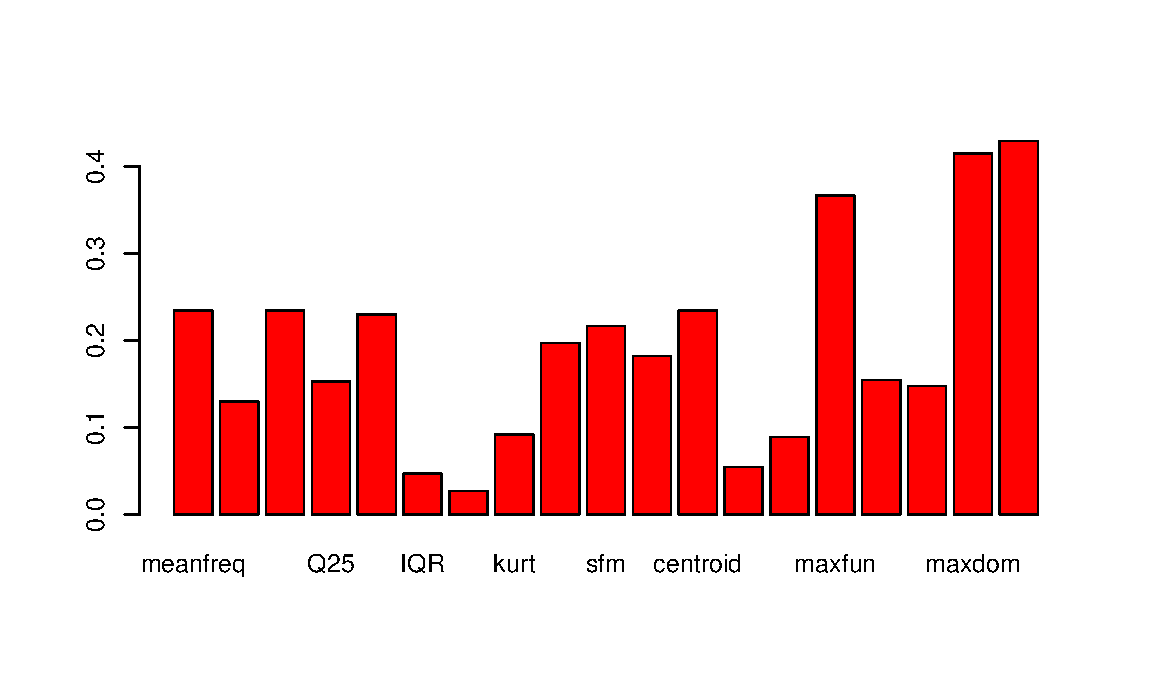
\includegraphics[width=\textwidth, height = 7.5cm]{Rplot_corr_target.eps}
\begin{verbatim}> library(corrplot)
> correlations = cor(dataTransScaled[, 1:(colnum - 1)])
> corrplot(correlations)
> round(correlations, 2)
         meanfreq    sd median   Q25   Q75   IQR  skew  kurt sp.ent   sfm  mode centroid
meanfreq     1.00 -0.74   0.92  0.91  0.73 -0.62 -0.14 -0.23  -0.64 -0.81  0.68     1.00
sd          -0.74  1.00  -0.55 -0.84 -0.15  0.87  0.02  0.09   0.74  0.85 -0.52    -0.74
median       0.92 -0.55   1.00  0.77  0.74 -0.46 -0.14 -0.22  -0.54 -0.68  0.67     0.92
Q25          0.91 -0.84   0.77  1.00  0.47 -0.86  0.00 -0.07  -0.69 -0.78  0.58     0.91
Q75          0.73 -0.15   0.74  0.47  1.00  0.03 -0.27 -0.34  -0.20 -0.39  0.49     0.73
IQR         -0.62  0.87  -0.46 -0.86  0.03  1.00 -0.17 -0.13   0.70  0.67 -0.38    -0.62
skew        -0.14  0.02  -0.14  0.00 -0.27 -0.17  1.00  0.96  -0.38 -0.09 -0.36    -0.14
kurt        -0.23  0.09  -0.22 -0.07 -0.34 -0.13  0.96  1.00  -0.27  0.02 -0.44    -0.23
sp.ent      -0.64  0.74  -0.54 -0.69 -0.20  0.70 -0.38 -0.27   1.00  0.88 -0.33    -0.64
sfm         -0.81  0.85  -0.68 -0.78 -0.39  0.67 -0.09  0.02   0.88  1.00 -0.49    -0.81
mode         0.68 -0.52   0.67  0.58  0.49 -0.38 -0.36 -0.44  -0.33 -0.49  1.00     0.68
centroid     1.00 -0.74   0.92  0.91  0.73 -0.62 -0.14 -0.23  -0.64 -0.81  0.68     1.00
meanfun      0.49 -0.49   0.44  0.58  0.16 -0.59  0.03  0.00  -0.51 -0.45  0.32     0.49
minfun       0.46 -0.39   0.41  0.36  0.34 -0.22 -0.24 -0.30  -0.33 -0.41  0.46     0.46
maxfun       0.32 -0.14   0.30  0.22  0.32 -0.07 -0.14 -0.18  -0.13 -0.21  0.18     0.32
meandom      0.56 -0.50   0.48  0.48  0.38 -0.33 -0.37 -0.41  -0.27 -0.44  0.55     0.56
mindom       0.33 -0.44   0.29  0.38  0.07 -0.40  0.01 -0.02  -0.34 -0.37  0.32     0.33
maxdom       0.53 -0.49   0.45  0.46  0.34 -0.32 -0.35 -0.40  -0.26 -0.42  0.52     0.53
dfrange      0.53 -0.48   0.45  0.46  0.34 -0.32 -0.26 -0.32  -0.32 -0.44  0.47     0.53
modindx     -0.23  0.13  -0.23 -0.15 -0.23  0.05  0.03  0.09   0.20  0.22 -0.18    -0.23
         meanfun minfun maxfun meandom mindom maxdom dfrange modindx
meanfreq    0.49   0.46   0.32    0.56   0.33   0.53    0.53   -0.23
sd         -0.49  -0.39  -0.14   -0.50  -0.44  -0.49   -0.48    0.13
median      0.44   0.41   0.30    0.48   0.29   0.45    0.45   -0.23
Q25         0.58   0.36   0.22    0.48   0.38   0.46    0.46   -0.15
Q75         0.16   0.34   0.32    0.38   0.07   0.34    0.34   -0.23
IQR        -0.59  -0.22  -0.07   -0.33  -0.40  -0.32   -0.32    0.05
skew        0.03  -0.24  -0.14   -0.37   0.01  -0.35   -0.26    0.03
kurt        0.00  -0.30  -0.18   -0.41  -0.02  -0.40   -0.32    0.09
sp.ent     -0.51  -0.33  -0.13   -0.27  -0.34  -0.26   -0.32    0.20
sfm        -0.45  -0.41  -0.21   -0.44  -0.37  -0.42   -0.44    0.22
mode        0.32   0.46   0.18    0.55   0.32   0.52    0.47   -0.18
centroid    0.49   0.46   0.32    0.56   0.33   0.53    0.53   -0.23
meanfun     1.00   0.33   0.31    0.28   0.15   0.27    0.28   -0.05
minfun      0.33   1.00   0.30    0.52   0.18   0.44    0.43   -0.09
maxfun      0.31   0.30   1.00    0.35  -0.20   0.37    0.38   -0.37
meandom     0.28   0.52   0.35    1.00   0.23   0.86    0.82   -0.15
mindom      0.15   0.18  -0.20    0.23   1.00   0.15    0.12    0.15
maxdom      0.27   0.44   0.37    0.86   0.15   1.00    0.96   -0.42
dfrange     0.28   0.43   0.38    0.82   0.12   0.96    1.00   -0.43
modindx    -0.05  -0.09  -0.37   -0.15   0.15  -0.42   -0.43    1.00
> removed.cols = findCorrelation(correlations)
> removed.cols
[1]  1 12 18  7
> nearZeroVar(dataTransScaled)
integer(0)
> \end{verbatim}
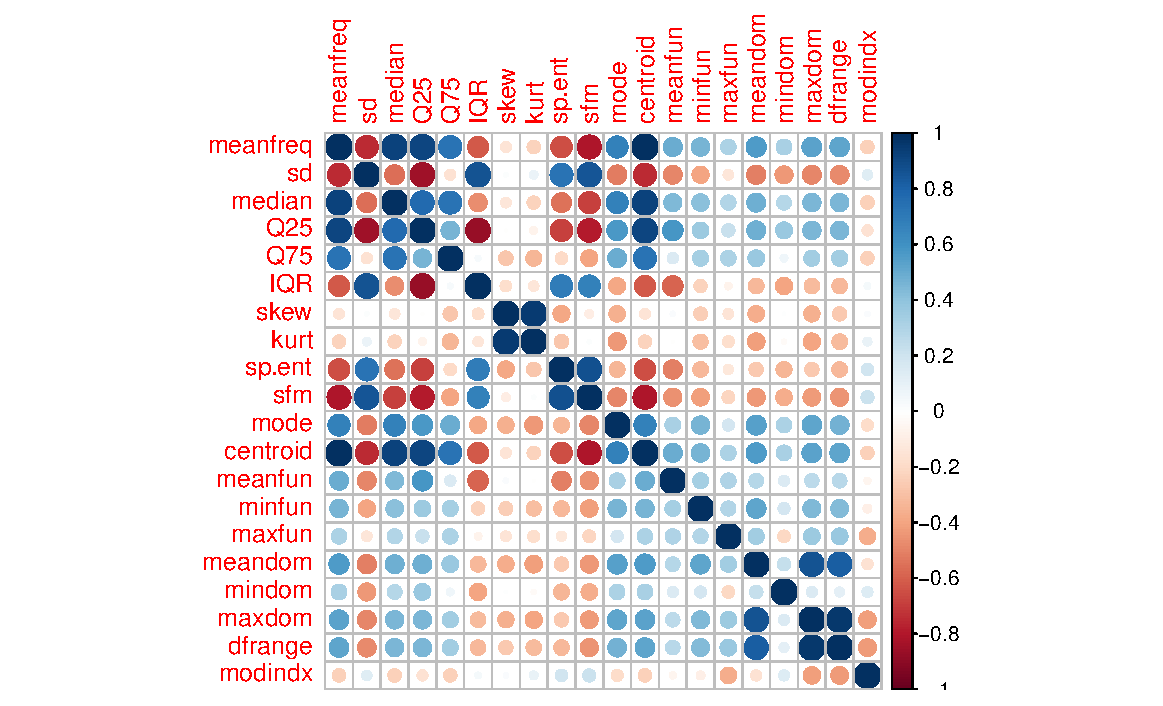
\includegraphics[width = \textwidth, height = 8cm]{Rplot_correlations.eps}
So there is no Almost-zero-variance-features, then we only need to remove some unnecessary features which are highly correlated to other features. Now we get the pre-procesed voice data and then we can begin to do the classification.
\begin{verbatim}
> dataProcessed.df = dataTransScaled[, -removed.cols]
> str(dataProcessed.df)
'data.frame':	3168 obs. of  17 variables:
 $ sd     : num  0.461 0.636 1.541 0.905 1.29 ...
 $ median : num  -2.815 -2.767 -2.789 -0.876 -1.639 ...
 $ Q25    : num  -2.246 -2.196 -2.311 -0.951 -1.283 ...
 $ Q75    : num  -4.215 -4.171 -3.306 -0.769 -0.846 ...
 $ IQR    : num  -0.0756 -0.1201 0.9211 0.6972 0.9965 ...
 $ kurt   : num  2.2 2.33 2.38 -1.33 -1.24 ...
 $ sp.ent : num  -0.0648 -0.0912 -1.0905 1.565 1.7747 ...
 $ sfm    : num  0.553 0.661 0.487 1.62 1.848 ...
 $ mode   : num  -2.14 -2.14 -2.14 -1.05 -0.79 ...
 $ meanfun: num  -1.81 -1.08 -1.37 -1.67 -1.13 ...
 $ minfun : num  -1.38 -1.37 -1.39 -1.14 -1.24 ...
 $ maxfun : num  0.602 -0.397 0.414 -0.397 0.236 ...
 $ meandom: num  -2.2204 -2.2067 -2.2184 -1.2976 -0.0774 ...
 $ mindom : num  -1.16 -1.16 -1.16 -1.16 -1.16 ...
 $ dfrange: num  -1.419 -1.406 -1.417 -1.261 0.137 ...
 $ modindx: num  -1.455 -1.014 -1.065 0.614 0.289 ...
 $ label  : Factor w/ 2 levels "female","male": 2 2 2 2 2 2 2 2 2 2 ...
> \end{verbatim}
\subsection{Logistic Regression}
First, we will use logistic regression to do the prediction.
\begin{verbatim}> gender.logistic = glm(label ~ ., data = dataProcessed.training, family = binomial)
> coef(gender.logistic)
 (Intercept)           sd       median          Q25          Q75          IQR
-1.056148334  0.563436060 -0.006193674 -0.241897964  0.139922568  1.735964645
        kurt       sp.ent          sfm         mode      meanfun       minfun
-0.014667841  1.267915881 -1.450901813  0.246825137 -5.568683495  0.965973200
      maxfun      meandom       mindom      dfrange      modindx
 0.165966989  0.046386559 -0.200657397  0.029098771 -0.039937984
> probs = predict(gender.logistic, type = "response")
> logistic.table = table(dataProcessed.training$label, probs > 0.5)
> logistic.table

         FALSE TRUE
  female  1088   25
  male      25 1079
>
> class.sensi = function(table) {
+   table[2,2] / sum(table[2,])
+ }
>
> class.speci = function(table) {
+   table[1,1] / sum(table[1,])
+ }
>
> total.error = function(table) {
+   1 - sum(diag(table)) / sum(table)
+ }
> class.sensi(logistic.table)
[1] 0.9773551
> class.speci(logistic.table)
[1] 0.9775382
> total.error(logistic.table)
[1] 0.022553
> \end{verbatim}
Now we would like to bootstrap and CV result, and verify the error on test data set.
\begin{verbatim}
> library(R330)
> logistic.cv10 = cross.val(gender.logistic, nfold = 10)
Mean Specificity =  0.9724298
Mean Sensitivity =  0.9755166
Mean Correctly classified =  0.9740045
> logistic.cv10.error = 1 - mean(logistic.cv10$Correct)
> logistic.cv10.error
[1] 0.02599548
>
> err.boot(gender.logistic, B = 200)
$err
[1] 0.022553

$Err
[1] 0.02240641

>
> logistic.CV5 = train(
+   label ~ .,
+   data = dataProcessed.training,
+   method = "glm",
+   trControl = trainControl(
+     method = "cv",
+     number = 5,
+     repeats = 20
+   )
+ )
Warning message:
`repeats` has no meaning for this resampling method.
>
> logistic.CV5
Generalized Linear Model

2217 samples
  16 predictor
   2 classes: 'female', 'male'

No pre-processing
Resampling: Cross-Validated (5 fold)
Summary of sample sizes: 1773, 1774, 1774, 1773, 1774
Resampling results:

  Accuracy   Kappa
  0.9733868  0.9467736

> 1 - logistic.CV5$results$Accuracy
[1] 0.02661318
>
> logistic.boot = train(
+   label ~ .,
+   data = dataProcessed.training,
+   method = "glm",
+   trControl = trainControl(method = "boot",
+                            repeats = 200)
+ )
Warning message:
`repeats` has no meaning for this resampling method.
>
> logistic.boot
Generalized Linear Model

2217 samples
  16 predictor
   2 classes: 'female', 'male'

No pre-processing
Resampling: Bootstrapped (25 reps)
Summary of sample sizes: 2217, 2217, 2217, 2217, 2217, 2217, ...
Resampling results:

  Accuracy   Kappa
  0.9733918  0.9467496

> 1 - logistic.boot$results$Accuracy
[1] 0.02660823
> 
> probs.test = predict(gender.logistic,
+                      type = "response",
+                      newdata = dataProcessed.test)
> logistic.table.test = table(dataProcessed.test$label,
+                             probs.test > 0.5)
> logistic.table.test

         FALSE TRUE
  female   458   13
  male      12  468
> class.sensi(logistic.table.test)
[1] 0.975
> class.speci(logistic.table.test)
[1] 0.9723992
> total.error(logistic.table.test)
[1] 0.02628812
> \end{verbatim}
\subsection{Linear Discriminant Analysis (LDA)}
Second, we will use LDA to do the prediction.
\begin{verbatim}> library(MASS)
> gender.lda = lda(label ~ ., data = dataProcessed.training)
> lda.prediction = predict(gender.lda)
> predClasses = lda.prediction$class
> head(predClasses)
[1] female female male   female male   female
Levels: female male
> lda.probs = lda.prediction$posterior
> head(lda.probs)
           female        male
1769 9.932484e-01 0.006751595
1619 6.619340e-01 0.338066037
328  1.447354e-05 0.999985526
2954 9.987365e-01 0.001263537
914  1.187965e-03 0.998812035
1934 9.864788e-01 0.013521166
>
> ldaTable = table(predClasses, dataProcessed.training$label)
> ldaTable

predClasses female male
     female   1073   20
     male       40 1084
>
> class.sensi(ldaTable)
[1] 0.9644128
> class.speci(ldaTable)
[1] 0.9817017
> total.error(ldaTable)
[1] 0.0270636
>
> lda.CV10 = train(
+   label ~ .,
+   data = dataProcessed.training,
+   method = "lda",
+   trControl = trainControl(
+     method = "cv",
+     number = 10,
+     repeats = 20
+   )
+ )
Warning message:
`repeats` has no meaning for this resampling method.
>
> lda.CV10
Linear Discriminant Analysis

2217 samples
  16 predictor
   2 classes: 'female', 'male'

No pre-processing
Resampling: Cross-Validated (10 fold)
Summary of sample sizes: 1994, 1996, 1995, 1995, 1996, 1995, ...
Resampling results:

  Accuracy   Kappa
  0.9720251  0.9440541

> 1 - lda.CV10$results$Accuracy
[1] 0.0279749
>
> lda.boot = train(
+   label ~ .,
+   data = dataProcessed.training,
+   method = "lda",
+   trControl = trainControl(method = "boot",
+                            repeats = 200)
+ )
Warning message:
`repeats` has no meaning for this resampling method.
>
> lda.boot
Linear Discriminant Analysis

2217 samples
  16 predictor
   2 classes: 'female', 'male'

No pre-processing
Resampling: Bootstrapped (25 reps)
Summary of sample sizes: 2217, 2217, 2217, 2217, 2217, 2217, ...
Resampling results:

  Accuracy   Kappa
  0.9718173  0.9435844

> 1 - lda.boot$results$Accuracy
[1] 0.0281827
> 
> prediction.test = predict(gender.lda,
+                           newdata = dataProcessed.test)
> predClasses.test = prediction.test$class
> lda.probs.test = prediction.test$posterior
> lda.table.test = table(predClasses.test,
+                        dataProcessed.test$label)
> lda.table.test

predClasses.test female male
          female    452   12
          male       19  468
>
> class.sensi(lda.table.test)
[1] 0.9609856
> class.speci(lda.table.test)
[1] 0.9741379
> total.error(lda.table.test)
[1] 0.03259727
> \end{verbatim}
\subsection{Quadratic Discriminant Analysis (QDA)}
Third, we will use QDA to make the prediction model.
\begin{verbatim}> gender.qda = qda(label ~ ., data = dataProcessed.training)
> qda.prediction = predict(gender.qda)
> predClasses = qda.prediction$class
> head(predClasses)
[1] female female male   female male   female
Levels: female male
> qda.probs = qda.prediction$posterior
> head(qda.probs)
           female         male
1769 9.271242e-01 7.287584e-02
1619 5.884286e-01 4.115714e-01
328  3.937558e-06 9.999961e-01
2954 9.999259e-01 7.411375e-05
914  4.954468e-05 9.999505e-01
1934 9.575210e-01 4.247903e-02
>
> qdaTable = table(predClasses, dataProcessed.training$label)
> qdaTable

predClasses female male
     female   1074   31
     male       39 1073
>
> class.sensi(qdaTable)
[1] 0.9649281
> class.speci(qdaTable)
[1] 0.9719457
> total.error(qdaTable)
[1] 0.0315742
>
> qda.CV10 = train(
+   label ~ .,
+   data = dataProcessed.training,
+   method = "qda",
+   trControl = trainControl(
+     method = "cv",
+     number = 10,
+     repeats = 20
+   )
+ )
Warning message:
`repeats` has no meaning for this resampling method.
>
> qda.CV10
Quadratic Discriminant Analysis

2217 samples
  16 predictor
   2 classes: 'female', 'male'

No pre-processing
Resampling: Cross-Validated (10 fold)
Summary of sample sizes: 1995, 1996, 1994, 1996, 1996, 1995, ...
Resampling results:

  Accuracy   Kappa
  0.9670742  0.9341472

> 1 - qda.CV10$results$Accuracy
[1] 0.03292583
>
> qda.boot = train(
+   label ~ .,
+   data = dataProcessed.training,
+   method = "qda",
+   trControl = trainControl(method = "boot",
+                            repeats = 200)
+ )
Warning message:
`repeats` has no meaning for this resampling method.
>
> qda.boot
Quadratic Discriminant Analysis

2217 samples
  16 predictor
   2 classes: 'female', 'male'

No pre-processing
Resampling: Bootstrapped (25 reps)
Summary of sample sizes: 2217, 2217, 2217, 2217, 2217, 2217, ...
Resampling results:

  Accuracy   Kappa
  0.9658119  0.931563

> 1 - qda.boot$results$Accuracy
[1] 0.03418807
> 
> prediction.test = predict(gender.qda,
+                           newdata = dataProcessed.test)
> predClasses.test = prediction.test$class
> qda.probs.test = prediction.test$posterior
> qda.table.test = table(predClasses.test,
+                        dataProcessed.test$label)
> qda.table.test

predClasses.test female male
          female    454   14
          male       17  466
>
> class.sensi(qda.table.test)
[1] 0.9648033
> class.speci(qda.table.test)
[1] 0.9700855
> total.error(qda.table.test)
[1] 0.03259727
> \end{verbatim}
\subsection{K-Nearest Neighbours (KNN)}
Forth, we will use k-nearest neighbours method to make the prediction model.
\begin{verbatim}> library(class)
> colnum = ncol(dataProcessed.training)
> dataProcessed.knn = data.frame(dataProcessed.training[,1:(colnum - 1)],
+                                label = as.numeric(dataProcessed.training[, colnum]))
> knn.prediction = knn(dataProcessed.knn,
+                      dataProcessed.knn,
+                      dataProcessed.knn$label,
+                      k = 5)
>
> knnTable = table(dataProcessed.training$label, knn.prediction)
> knnTable
        knn.prediction
            1    2
  female 1103   10
  male      6 1098
>
> class.sensi(knnTable)
[1] 0.9945652
> class.speci(knnTable)
[1] 0.9910153
> total.error(knnTable)
[1] 0.00721696
>
> knn.CV10 = train(
+   label ~ .,
+   data = dataProcessed.training,
+   method = "knn",
+   trControl = trainControl(
+     method = "cv",
+     number = 10,
+     repeats = 20
+   )
+ )
Warning message:
`repeats` has no meaning for this resampling method.
>
> knn.CV10
k-Nearest Neighbors

2217 samples
  16 predictor
   2 classes: 'female', 'male'

No pre-processing
Resampling: Cross-Validated (10 fold)
Summary of sample sizes: 1995, 1996, 1996, 1995, 1996, 1995, ...
Resampling results across tuning parameters:

  k  Accuracy   Kappa
  5  0.9715828  0.9431693
  7  0.9684255  0.9368565
  9  0.9657309  0.9314705

Accuracy was used to select the optimal model using  the largest value.
The final value used for the model was k = 5.
> 1 - knn.CV10$results$Accuracy
[1] 0.02841721 0.03157446 0.03426907
>
> knn.boot = train(
+   label ~ .,
+   data = dataProcessed.training,
+   method = "knn",
+   trControl = trainControl(method = "boot",
+                            repeats = 200)
+ )
Warning message:
`repeats` has no meaning for this resampling method.
>
> knn.boot
k-Nearest Neighbors

2217 samples
  16 predictor
   2 classes: 'female', 'male'

No pre-processing
Resampling: Bootstrapped (25 reps)
Summary of sample sizes: 2217, 2217, 2217, 2217, 2217, 2217, ...
Resampling results across tuning parameters:

  k  Accuracy   Kappa
  5  0.9669217  0.9338148
  7  0.9668513  0.9336702
  9  0.9653298  0.9306300

Accuracy was used to select the optimal model using  the largest value.
The final value used for the model was k = 5.
> 1 - knn.boot$results$Accuracy
[1] 0.03307826 0.03314867 0.03467020
> 
> dataProcessed.knn.test = data.frame(dataProcessed.test[, 1:(colnum - 1)],
+                                     label = as.numeric(dataProcessed.test[, colnum]))
> knn.prediction.test = knn(dataProcessed.knn,
+                           dataProcessed.knn.test,
+                           dataProcessed.knn$label,
+                           k = 5)
>
> knnTable.test = table(dataProcessed.test$label, knn.prediction.test)
> knnTable.test
        knn.prediction.test
           1   2
  female 464   7
  male     8 472
>
> class.sensi(knnTable.test)
[1] 0.9833333
> class.speci(knnTable.test)
[1] 0.985138
> total.error(knnTable.test)
[1] 0.01577287
> \end{verbatim}
\subsection{Additive Model (GAM)}
Fifth, we will use additive model to make the prediction model.
\begin{verbatim}> library(mgcv)
> gender.gam = gam(label ~ s(sd) + s(median) + s(Q25)
+                  + s(Q75) + s(IQR) + s(kurt) + s(sp.ent)
+                  + s(sfm) + s(mode) + s(meanfun) + s(minfun)
+                  + s(maxfun) + s(meandom) + s(mindom)
+                  + s(dfrange) + s(modindx),
+                  data = dataProcessed.training,
+                  family = binomial)
> par(mfrow = c(2, 2))
> plot(gender.gam)
Hit <Return> to see next plot: gam.probs = predict(gender.gam, type = "response")
Hit <Return> to see next plot: gam.table = table(dataProcessed.df$label, gam.probs > 0.5)
Hit <Return> to see next plot: gam.table
Hit <Return> to see next plot:
> class.sensi(gam.table)
[1] 0.9873737
> class.speci(gam.table)
[1] 0.9905303
> total.error(gam.table)
[1] 0.01104798
> 
> gam.probs.test = predict(gender.gam,
+                          type = "response",
+                          newdata = dataProcessed.test)
> gam.table.test = table(dataProcessed.test$label,
+                        gam.probs.test > 0.5)
> gam.table.test

         FALSE TRUE
  female   462    9
  male      12  468
>
> class.sensi(gam.table.test)
[1] 0.975
> class.speci(gam.table.test)
[1] 0.9808917
> total.error(gam.table.test)
[1] 0.02208202
> \end{verbatim}
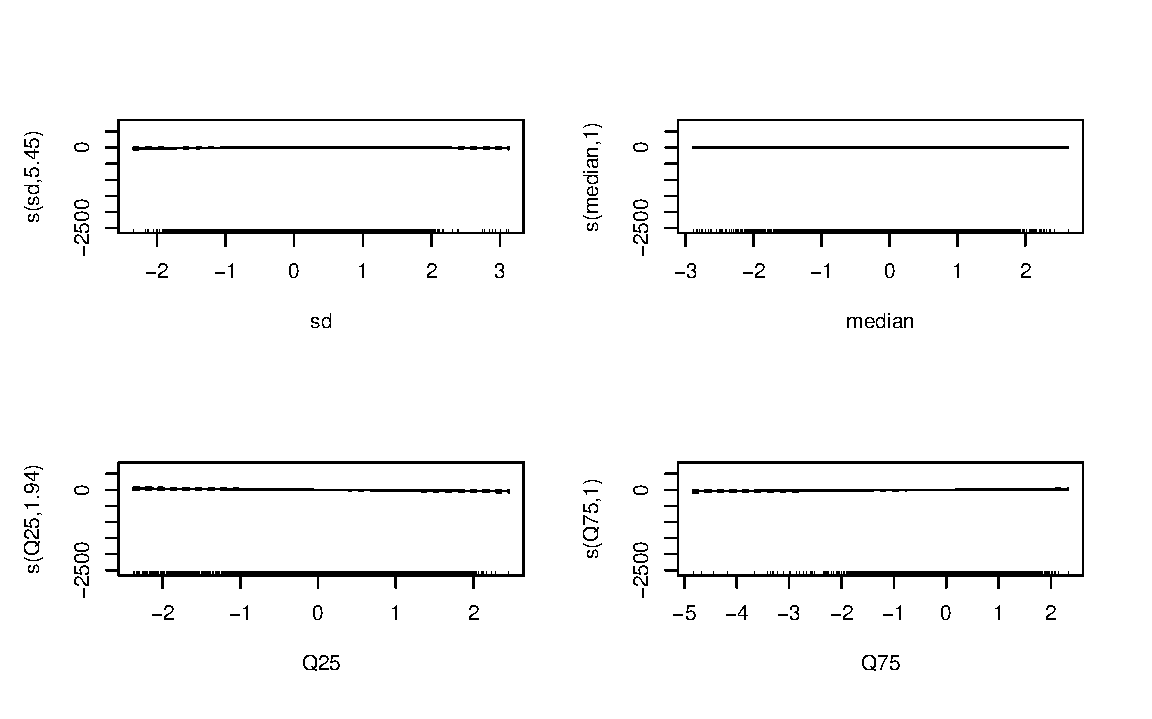
\includegraphics[width = \textwidth, height = 8.5cm]{Rplot_gam_1.eps}

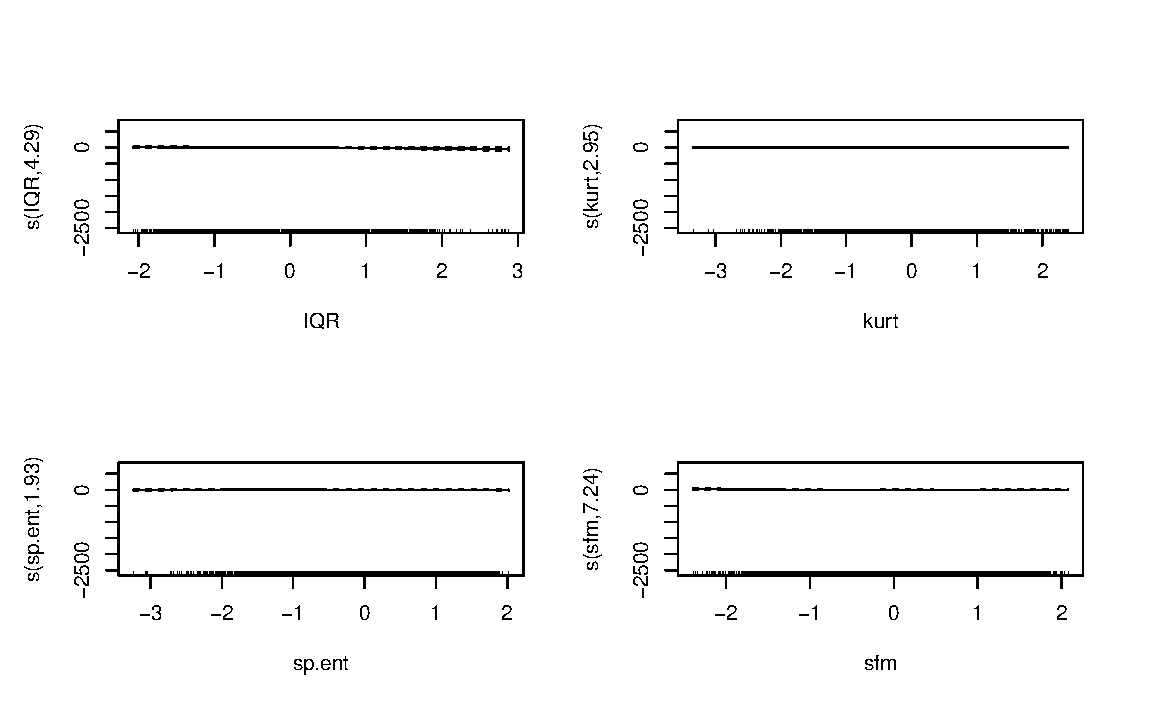
\includegraphics[width = \textwidth, height = 8.5cm]{Rplot_gam_2.eps}

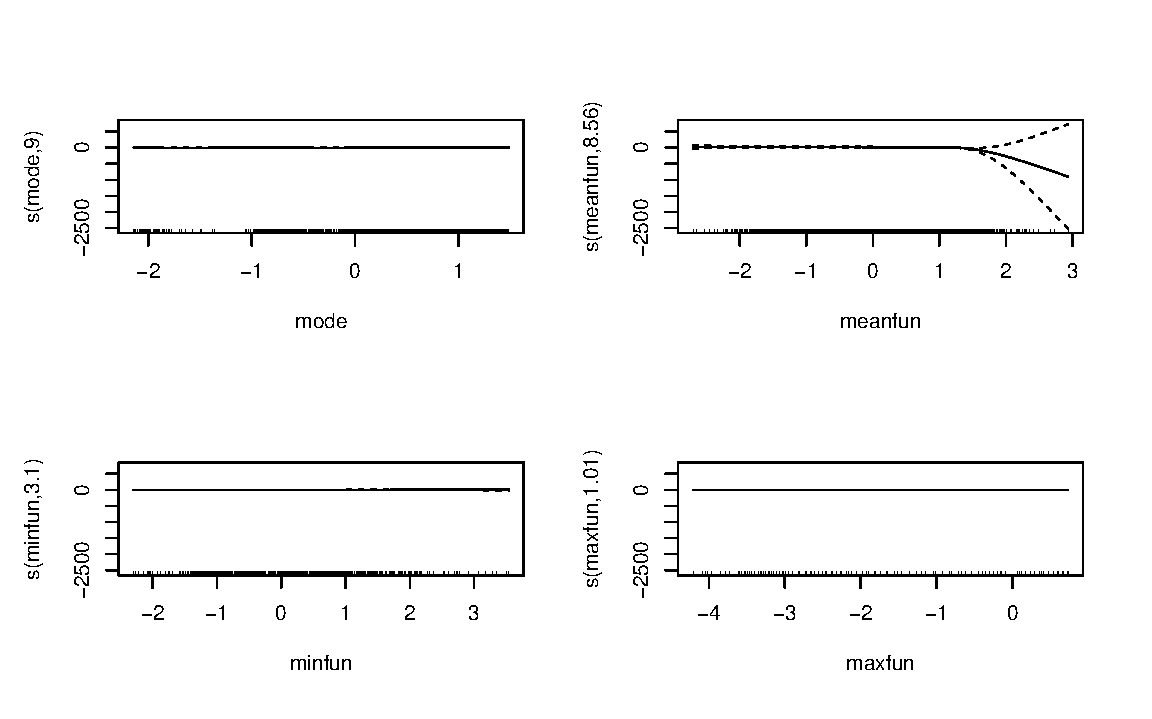
\includegraphics[width = \textwidth]{Rplot_gam_3.eps}

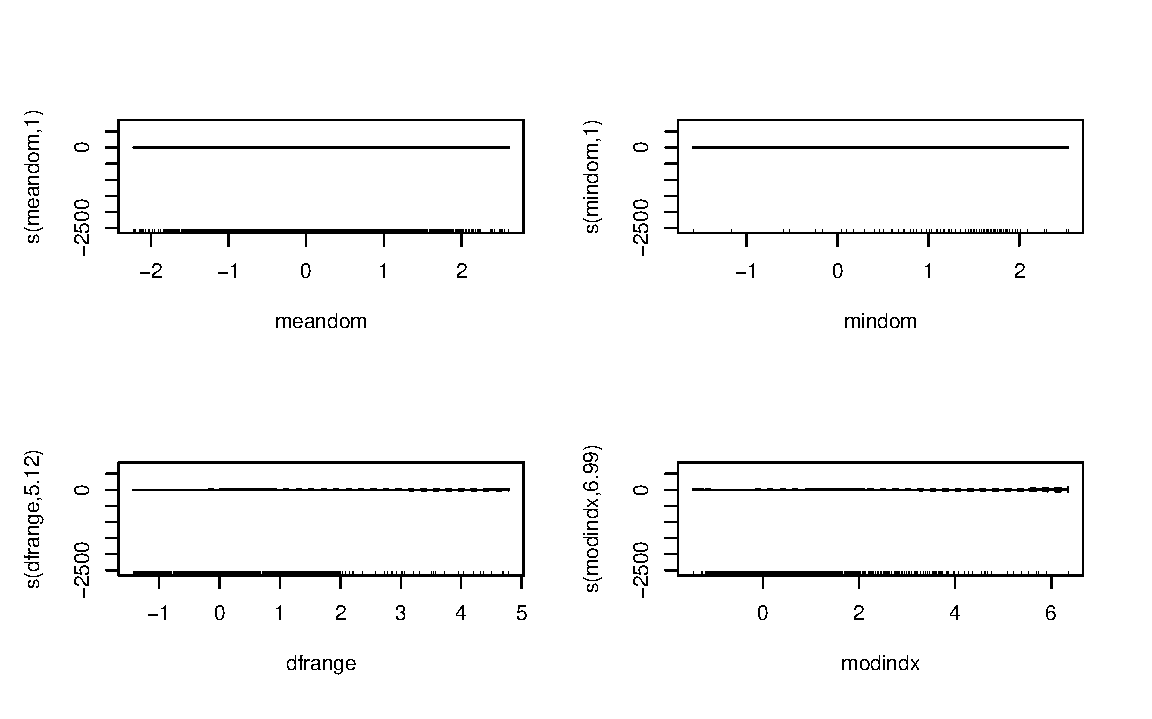
\includegraphics[width = \textwidth]{Rplot_gam_4.eps}
\subsection{Neural Network (NNET)}
Sixth, we will use Neural network to make the prediction model.
\begin{verbatim}> my.grid = expand.grid(.decay = c(0.01, 0.001), .size = c(4, 6, 8))
> nn.CV = train(label ~ .,
+               data = dataProcessed.training,
+               method = "nnet",
+               maxit = 1000,
+               tuneGrid = my.grid,
+               trace = FALSE,
+               trControl = trainControl(method = "cv",
+                                        number = 10,
+                                        repeats = 100))

Attaching package: ‘nnet’

The following object is masked from ‘package:mgcv’:

    multinom

Warning message:
`repeats` has no meaning for this resampling method.
>
> nn.CV
Neural Network

2217 samples
  16 predictor
   2 classes: 'female', 'male'

No pre-processing
Resampling: Cross-Validated (10 fold)
Summary of sample sizes: 1996, 1995, 1995, 1996, 1995, 1995, ...
Resampling results across tuning parameters:

  decay  size  Accuracy   Kappa
  0.001  4     0.9706819  0.9413594
  0.001  6     0.9638885  0.9277743
  0.001  8     0.9634523  0.9269039
  0.010  4     0.9684195  0.9368352
  0.010  6     0.9639088  0.9278090
  0.010  8     0.9715787  0.9431545

Accuracy was used to select the optimal model using  the largest value.
The final values used for the model were size = 8 and decay = 0.01.
> 1 - nn.CV$results$Accuracy[nn.CV$results$size == 8 & nn.CV$results$decay == 0.01]
[1] 0.02842127
> library(nnet)
> nnet.fit = nnet(label ~ .,
+                 data = dataProcessed.training,
+                 size = 8,
+                 decay = 0.01,
+                 maxit = 1000)
# weights:  145
initial  value 1601.138259
iter  10 value 171.114006
iter  20 value 120.222933
iter  30 value 78.348856
iter  40 value 57.276961
iter  50 value 50.394225
......  .......  .......
iter 300 value 21.937532
iter 310 value 21.936938
iter 320 value 21.936633
iter 330 value 21.936564
final  value 21.936559
converged
>
> summary(nnet.fit)
a 16-8-1 network with 145 weights
options were - entropy fitting  decay=0.01
  b->h1  i1->h1  i2->h1  i3->h1  i4->h1  i5->h1  i6->h1  i7->h1  i8->h1  i9->h1 i10->h1
   0.59    1.52    1.65   -4.12   -2.61    4.13    0.28   -2.26    1.27    1.38    3.05
i11->h1 i12->h1 i13->h1 i14->h1 i15->h1 i16->h1
   0.23   -0.66   -1.40   -0.38    0.68   -0.15
  b->h2  i1->h2  i2->h2  i3->h2  i4->h2  i5->h2  i6->h2  i7->h2  i8->h2  i9->h2 i10->h2
   2.30   -5.50    4.40   -0.57   -5.13   -0.48    0.14   -0.59    1.76   -0.16    1.00
i11->h2 i12->h2 i13->h2 i14->h2 i15->h2 i16->h2
   0.13    1.28    2.91    1.02    0.10   -2.21
  b->h3  i1->h3  i2->h3  i3->h3  i4->h3  i5->h3  i6->h3  i7->h3  i8->h3  i9->h3 i10->h3
  -4.22   -7.64   -0.15    1.63    0.57    0.35   -1.16   -0.15    2.60    0.95    2.66
i11->h3 i12->h3 i13->h3 i14->h3 i15->h3 i16->h3
   0.53    3.03   -1.41   -0.67    0.69   -2.30
  b->h4  i1->h4  i2->h4  i3->h4  i4->h4  i5->h4  i6->h4  i7->h4  i8->h4  i9->h4 i10->h4
   0.27   -3.05    0.13   -0.14    0.32    0.68   -4.89   -1.24    0.84    1.62    2.84
i11->h4 i12->h4 i13->h4 i14->h4 i15->h4 i16->h4
  -1.76    1.03    1.77   -2.64   -3.54    0.51
  b->h5  i1->h5  i2->h5  i3->h5  i4->h5  i5->h5  i6->h5  i7->h5  i8->h5  i9->h5 i10->h5
  -4.85   -1.40   -1.44   -0.03   -1.00   -0.14    0.20   -2.90    0.48    1.28   -1.40
i11->h5 i12->h5 i13->h5 i14->h5 i15->h5 i16->h5
  -1.39    0.76    0.46   -3.76   -0.53   -1.62
  b->h6  i1->h6  i2->h6  i3->h6  i4->h6  i5->h6  i6->h6  i7->h6  i8->h6  i9->h6 i10->h6
   1.02   -1.93    3.17   -1.30   -1.19   -1.45   -0.33    1.94    0.39   -0.91    8.56
i11->h6 i12->h6 i13->h6 i14->h6 i15->h6 i16->h6
  -1.38   -1.22   -0.57    1.20    1.62   -0.46
  b->h7  i1->h7  i2->h7  i3->h7  i4->h7  i5->h7  i6->h7  i7->h7  i8->h7  i9->h7 i10->h7
  -1.36    3.52   -1.85   -1.12   -0.23   -1.34    0.19    0.87    0.70    2.40    5.93
i11->h7 i12->h7 i13->h7 i14->h7 i15->h7 i16->h7
  -1.02   -1.66    0.26    0.21   -1.42    1.33
  b->h8  i1->h8  i2->h8  i3->h8  i4->h8  i5->h8  i6->h8  i7->h8  i8->h8  i9->h8 i10->h8
  -3.71   -1.49   -2.14    0.29    1.20    1.44    0.82    2.33   -2.03   -0.78   -5.14
i11->h8 i12->h8 i13->h8 i14->h8 i15->h8 i16->h8
   0.33   -0.94   -0.99    1.12    1.74   -0.61
  b->o  h1->o  h2->o  h3->o  h4->o  h5->o  h6->o  h7->o  h8->o
 -1.88   9.53  10.54 -13.67   9.12  -7.47 -12.92  -9.53  12.09
> nnet.probs = predict(nnet.fit)
> nnet.table.training = table(dataProcessed.training$label,
+                             nnet.probs > 0.5)
> nnet.table.training

         FALSE TRUE
  female  1113    0
  male       0 1104
>
> class.sensi(nnet.table.training)
[1] 1
> class.speci(nnet.table.training)
[1] 1
> total.error(nnet.table.training)
[1] 0
> nnet.probs.test = predict(nnet.fit, newdata = dataProcessed.test)
> nnet.table.test = table(dataProcessed.test$label,
+                         nnet.probs.test > 0.5)
> nnet.table.test

         FALSE TRUE
  female   452   19
  male      14  466
>
> class.sensi(nnet.table.test)
[1] 0.9708333
> class.speci(nnet.table.test)
[1] 0.9596603
> total.error(nnet.table.test)
[1] 0.03470032
> \end{verbatim}
\subsection{Classification Tree}
Seventh, we will use Classification Tree to make the prediction model. At first we use CV and bootstrap method to find the best CP value. And then use it to build the prediction model.
\begin{verbatim}> library(rpart)
> CV10.rpart = train(label ~ .,
+                    data = dataProcessed.training,
+                    method = "rpart",
+                    tuneLength = 200,
+                    trControl = trainControl(method = "cv",
+                                             number = 10,
+                                             repeats = 100))
Warning message:
`repeats` has no meaning for this resampling method.
> CV10.rpart
CART

2217 samples
  16 predictor
   2 classes: 'female', 'male'

No pre-processing
Resampling: Cross-Validated (10 fold)
Summary of sample sizes: 1995, 1996, 1994, 1994, 1996, 1995, ...
Resampling results across tuning parameters:

  cp           Accuracy   Kappa
  0.000000000  0.9675306  0.9350538
  0.004579055  0.9675408  0.9350801
  ...........  .........  .........
  0.906652829  0.9508414  0.9016847
  0.911231884  0.7659469  0.5305429

Accuracy was used to select the optimal model using  the largest value.
The final value used for the model was cp = 0.004579055.
>
> 1 - CV10.rpart$results$Accuracy[abs(CV10.rpart$results$cp - 0.004579055) < 1e-09]
[1] 0.03245924
> boot.rpart = train(label ~ .,
+                    data = dataProcessed.training,
+                    method = "rpart",
+                    tuneLength = 200,
+                    trControl = trainControl(method = "boot",
+                                             repeats = 200))
Warning message:
`repeats` has no meaning for this resampling method.
> boot.rpart
CART

2217 samples
  16 predictor
   2 classes: 'female', 'male'

No pre-processing
Resampling: Bootstrapped (25 reps)
Summary of sample sizes: 2217, 2217, 2217, 2217, 2217, 2217, ...
Resampling results across tuning parameters:

  cp           Accuracy   Kappa
  0.000000000  0.9644858  0.9289113
  0.004579055  0.9664720  0.9328728
  ...........  .........  .........
  0.906652829  0.7824555  0.5761244
  0.911231884  0.7255688  0.4659058

Accuracy was used to select the optimal model using  the largest value.
The final value used for the model was cp = 0.004579055.
>
> 1 - boot.rpart$results$Accuracy[abs(boot.rpart$results$cp - 0.004579055) < 1e-09]
[1] 0.03352798
> tree.fit.training = rpart(label ~ .,
+                  data = dataProcessed.training,
+                  method = "class",
+                  parms = list(split = "gini"),
+                  cp = 0.0046)
>
> par(mfrow = c(1, 1))
> plotcp(tree.fit.training)
> plot(tree.fit.training)
> text(tree.fit.training, cex = 0.7)
> printcp(tree.fit.training)

Classification tree:
rpart(formula = label ~ ., data = dataProcessed.training, method = "class",
    parms = list(split = "gini"), cp = 0.0046)

Variables actually used in tree construction:
[1] IQR     meanfun sp.ent

Root node error: 1104/2217 = 0.49797

n= 2217

         CP nsplit rel error   xerror      xstd
1 0.9112319      0  1.000000 1.038949 0.0213119
2 0.0095109      1  0.088768 0.098732 0.0092214
3 0.0076993      3  0.069746 0.081522 0.0084169
4 0.0054348      5  0.054348 0.066123 0.0076107
5 0.0046000      6  0.048913 0.064312 0.0075092
> \end{verbatim}
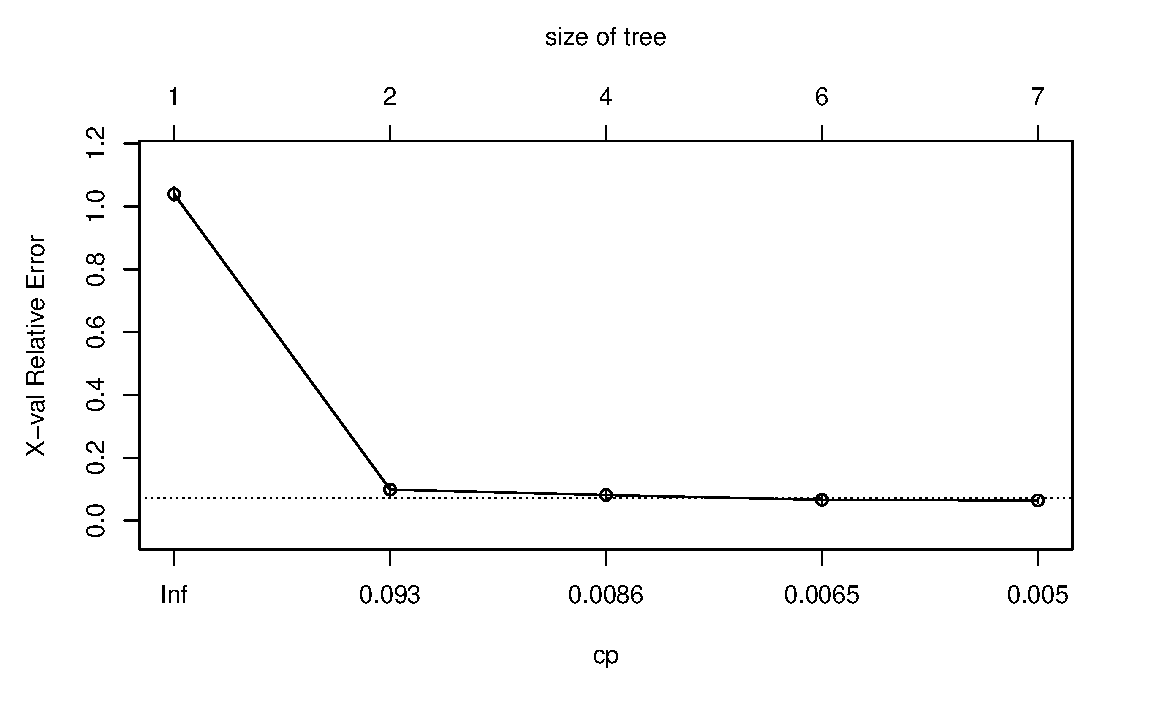
\includegraphics[width = \textwidth, height = 8.5cm]{Rplot_tree.eps}

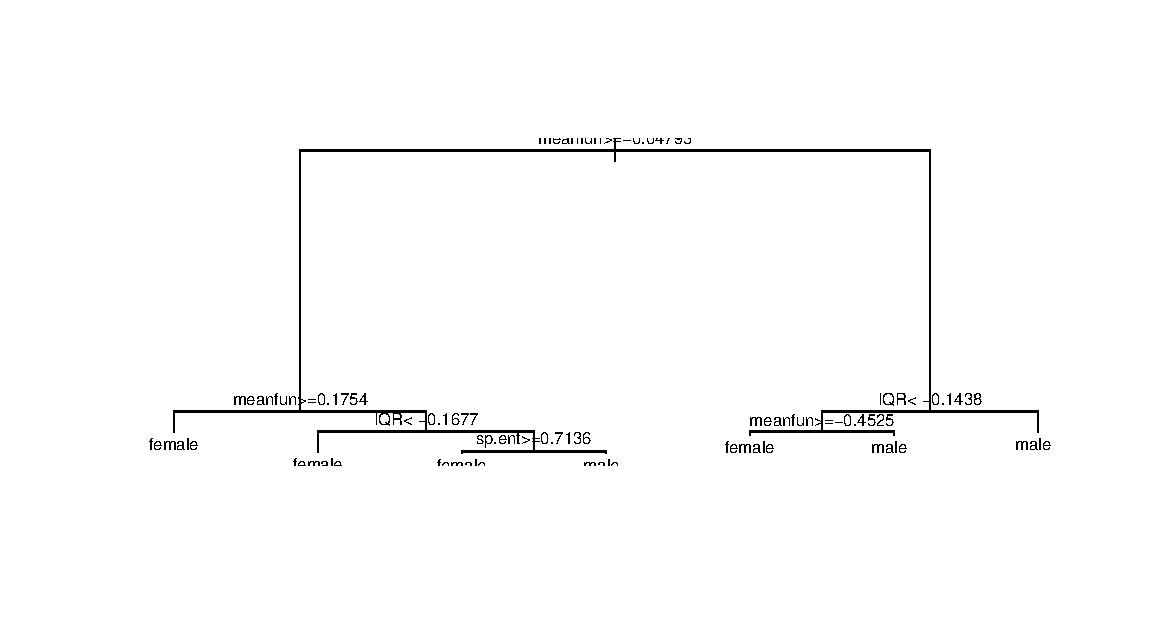
\includegraphics[width = \textwidth, height = 8.5cm]{Rplot_tree_branch.eps}
Then we calculate the training and test error of tree model.
\begin{verbatim}> tree.probs = predict(tree.fit.training)
> tree.table = table(dataProcessed.training$label, tree.probs[,2] > 0.5)
> tree.table

         FALSE TRUE
  female  1083   30
  male      24 1080
>
> class.sensi(tree.table)
[1] 0.9782609
> class.speci(tree.table)
[1] 0.9730458
> total.error(tree.table)
[1] 0.02435724
>
> tree.probs.test = predict(tree.fit.training, newdata = dataProcessed.test)
> tree.table.test = table(dataProcessed.test$label, tree.probs.test[,2] > 0.5)
> tree.table.test

         FALSE TRUE
  female   457   14
  male      17  463
>
> class.sensi(tree.table.test)
[1] 0.9645833
> class.speci(tree.table.test)
[1] 0.970276
> total.error(tree.table.test)
[1] 0.03259727
> \end{verbatim}
\subsection{Support Vector Machine (SVM)}
Eighth, we will use Support Vector Machine to make the prediction model. Using ksvm function we could get the training error and CV error, and then we could get test error on test data set.
\begin{verbatim}> library(kernlab)
> svm.stuff1.training = ksvm(
+   label ~ .,
+   data = dataProcessed.training,
+   C = 1,
+   cross = 5
+ )
> svm.stuff2.training = ksvm(
+   label ~ .,
+   data = dataProcessed.training,
+   C = 2,
+   cross = 10
+ )
> svm.stuff5.training = ksvm(
+   label ~ .,
+   data = dataProcessed.training,
+   C = 5,
+   cross = 10
+ )
>
> svm.stuff1.training
Support Vector Machine object of class "ksvm"

SV type: C-svc  (classification)
 parameter : cost C = 1

Gaussian Radial Basis kernel function.
 Hyperparameter : sigma =  0.0609944246877721

Number of Support Vectors : 299

Objective Function Value : -169.9957
Training error : 0.014885
Cross validation error : 0.019847
> svm.stuff2.training
Support Vector Machine object of class "ksvm"

SV type: C-svc  (classification)
 parameter : cost C = 2

Gaussian Radial Basis kernel function.
 Hyperparameter : sigma =  0.0611732542167164

Number of Support Vectors : 267

Objective Function Value : -259.1239
Training error : 0.011276
Cross validation error : 0.018038
> svm.stuff5.training
Support Vector Machine object of class "ksvm"

SV type: C-svc  (classification)
 parameter : cost C = 5

Gaussian Radial Basis kernel function.
 Hyperparameter : sigma =  0.0599590067580663

Number of Support Vectors : 239

Objective Function Value : -436.8405
Training error : 0.006315
Cross validation error : 0.018945
> svm.probs.test = predict(svm.stuff5.training, newdata = dataProcessed.test)
> svm.table.test = table(dataProcessed.test$label, svm.probs.test == "male")
> svm.table.test

         FALSE TRUE
  female   464    7
  male       9  471
>
> class.sensi(svm.table.test)
[1] 0.98125
> class.speci(svm.table.test)
[1] 0.985138
> total.error(svm.table.test)
[1] 0.0168244
> \end{verbatim}
\subsection{Gradient Boosting}
Ninth, we will use Gradient Boosting method to make the prediction model. This model in fact creates a boosting tree for the prediction.
\begin{verbatim}> library(mboost)
> colnum = ncol(dataProcessed.training)
> boost.tree = label ~ btree(dataProcessed.training[, -colnum],
+                      tree_controls = party::ctree_control(maxdepth = 4))
> gender.boost = mboost(
+   boost.tree,
+   data = dataProcessed.training,
+   family = Binomial(),
+   control = boost_control(mstop = 200, nu = 0.1)
+ )
> myrisk = cvrisk(gender.boost)
> myrisk

	 Cross-validated Negative Binomial Likelihood (logit link)
	 mboost(formula = boost.tree, data = dataProcessed.training, family = Binomial(),      control = boost_control(mstop = 250, nu = 0.1))

         0          1          2          3          4          5          6          7
0.69368678 0.57175609 0.48248919 0.41607134 0.36545716 0.32640449 0.29541790 0.27050572
.......... .......... .......... .......... .......... .........  .........   .........
       240        241        242        243        244        245        246        247
0.08699684 0.08698977 0.08698459 0.08698449 0.08696656 0.08696126 0.08696129 0.08695782
       248        249        250
0.08695430 0.08695588 0.08695550

	 Optimal number of boosting iterations: 248 
>
> boost.probs = predict(gender.boost)
> boost.table = table(dataProcessed.training$label,
+                     boost.probs > 0.5)
> boost.table

         FALSE TRUE
  female  1108    5
  male      29 1075
> class.sensi(boost.table)
[1] 0.9737319
> class.speci(boost.table)
[1] 0.9955076
> total.error(boost.table)
[1] 0.01533604
> boost.probs.test = predict(gender.boost, newdata = dataProcessed.test)
> boost.table.test = table(dataProcessed.test$label,
+                     boost.probs.test > 0.5)
> boost.table.test

         FALSE TRUE
  female   466    5
  male      16  464
>
> class.sensi(boost.table.test)
[1] 0.9666667
> class.speci(boost.table.test)
[1] 0.9893843
> total.error(boost.table.test)
[1] 0.02208202
> \end{verbatim}
\subsection{Random Forest}
Tenth, we will use Random Forest method to make the prediction model.
\begin{verbatim}> library(randomForest)
> gender.rf = randomForest(
+   label ~ .,
+   data = dataProcessed.training,
+   mtry = 10,
+   ntree = 1000
+ )
>
> plot(gender.rf)
> tail(gender.rf$err.rate, n = 2)
               OOB     female       male
 [999,] 0.02390618 0.02246181 0.02536232
[1000,] 0.02390618 0.02246181 0.02536232
> rf.probs = predict(gender.rf)
> rf.table = table(dataProcessed.training$label,
+                     rf.probs)
> rf.table
        rf.probs
         female male
  female   1088   25
  male       28 1076
> class.sensi(boost.table)
[1] 0.9737319
> class.speci(boost.table)
[1] 0.9955076
> total.error(boost.table)
[1] 0.01533604
> rf.probs.test = predict(gender.rf, newdata = dataProcessed.test)
> rf.table.test = table(dataProcessed.test$label,
+                       rf.probs.test)
> rf.table.test
        rf.probs.test
         female male
  female    463    8
  male       12  468
>
> class.sensi(rf.table.test)
[1] 0.975
> class.speci(rf.table.test)
[1] 0.9830149
> total.error(rf.table.test)
[1] 0.02103049
> \end{verbatim}

\includegraphics[width = \textwidth]{Rplot_random_forest.eps}
\subsection{Ridge Regression}
Eleventh, we will use Ridge Regression technique to make the prediction model.
\begin{verbatim}> library(glmnet)
> colnum = ncol(dataProcessed.training)
> X = as.matrix(dataProcessed.training[, -colnum])
> y = dataProcessed.training$label
> lambda.seq = seq(0.1, 0.001, length = 100)
> 
> gender.ridge = glmnet(X, y, alpha = 0, lambda = lambda.seq, family = "binomial")
> ridgecv = cv.glmnet(X, y, lambda = lambda.seq, family = "binomial")
> Pred.err.cv = ridgecv$cvm[ridgecv$lambda == ridgecv$lambda.min]
> Pred.err.cv
[1] 0.1843839
> 
> ridge.probs = predict(gender.ridge, X, type = "response")
> ridge.table = table(dataProcessed.training$label,
+                     ridge.probs[, length(ridgecv$cvm)] > 0.5)
> ridge.table

         FALSE TRUE
  female  1084   29
  male      23 1081
>
> class.sensi(ridge.table)
[1] 0.9791667
> class.speci(ridge.table)
[1] 0.9739443
> total.error(ridge.table)
[1] 0.02345512
>
> newX = as.matrix(dataProcessed.test[, -colnum])
> ridge.probs.test = predict(gender.ridge, newX, type = "response")
> ridge.table.test = table(dataProcessed.test$label,
+                     ridge.probs.test[, length(ridgecv$cvm)] > 0.5)
> ridge.table.test

         FALSE TRUE
  female   457   14
  male      12  468
>
> class.sensi(ridge.table.test)
[1] 0.975
> class.speci(ridge.table.test)
[1] 0.970276
> total.error(ridge.table.test)
[1] 0.02733964
> \end{verbatim}
\subsection{Lasso}
Twelfth, we will use lasso technique to make the prediction model.
\begin{verbatim}> gender.lasso = glmnet(X, y, alpha = 1, family = "binomial")
> lassocv = cv.glmnet(
+   X,
+   y,
+   lambda = gender.lasso$lambda,
+   family = "binomial",
+   type.measure = "class"
+ )
>
> plot(lassocv)
> lasso.err = lassocv$cvm[lassocv$lambda ==
+                           lassocv$lambda.min]
> lasso.err
[1] 0.02345512
> 
> lasso.probs = predict(gender.lasso, X)
> lasso.table = table(dataProcessed.training$label,
+                     lasso.probs[, length(lassocv$cvm)] > 0.5)
> lasso.table

         FALSE TRUE
  female  1094   19
  male      34 1070
>
> class.sensi(lasso.table)
[1] 0.9692029
> class.speci(lasso.table)
[1] 0.982929
> total.error(lasso.table)
[1] 0.02390618
> newX = as.matrix(dataProcessed.test[, -colnum])
> lasso.probs.test = predict(gender.lasso, newX)
> lasso.table.test = table(dataProcessed.test$label,
+                          lasso.probs.test[, length(lassocv$cvm)] > 0.5)
> lasso.table.test

         FALSE TRUE
  female   461   10
  male      17  463
>
> class.sensi(lasso.table.test)
[1] 0.9645833
> class.speci(lasso.table.test)
[1] 0.9787686
> total.error(lasso.table.test)
[1] 0.02839117
> \end{verbatim}
\subsection{Compare with all the techniques}
We have used 12 techniques to do the classification prediction based on the pre-processed data set. The results of the training error and test error are listed in the below table. \\
\setlength\extrarowheight{2pt}
\begin{tabular*}{\textwidth}{|l @{\extracolsep\fill}|c |c |c |c |}
  \hline
  % after \\: \hline or \cline{col1-col2} \cline{col3-col4} ...
  Model & training error & CV error & bootstrap error & test error \\
  \hline 
  logistic & 0.022553 & 0.02599548 & 0.022553 & 0.02628812 \\
  LDA & 0.0270636 & 0.0279749 & 0.0281827 & 0.03259727 \\
  QDA & 0.0315742 & 0.03292583 & 0.03418807 & 0.03259727 \\
  KNN & 0.00721696 & 0.02841721 & 0.03307826 & 0.01577287 \\
  GAM & 0.01104798 &  &  & 0.02208202 \\
  NNET & 0 & 0.02842127 &  & 0.03470032 \\
  TREE & 0.02435724 & 0.03245924 & 0.03352798 & 0.03259727 \\
  SVM & 0.006315 & 0.018945 &  & 0.0168244 \\
  Boost & 0.01533604 &  &  & 0.02208202 \\
  Random Forest & 0.01533604 & 0.02390618 (OOB) &  & 0.02103049 \\
  Ridge & 0.02345512 & 0.1843839 &  & 0.02733964 \\
  Lasso & 0.02390618 & 0.02345512 &  & 0.02839117 \\
  \hline
\end{tabular*}
\paragraph{}
From the table above, \textbf{it is obviously that KNN and SVM have the best test prediction error}, and SVM has much better training error than others including KNN. In addition, Random Forest and GAM and Gradient Boost also have good result than the others except KNN and SVM. The reason should be because all the features of the voice data are much more distributed and using function to fit them is difficult. \\
\indent There is a very interesting event that NNET has zero training error but the test error is a little higher. Obviously NNET makes a over-fitting for this voice data.\\
\indent So finally we choose \textbf{SVM and KNN} as the best choice of the techniques we have used for prediction.
\end{document}
